\begin{figure}[ht]   
\begin{center}
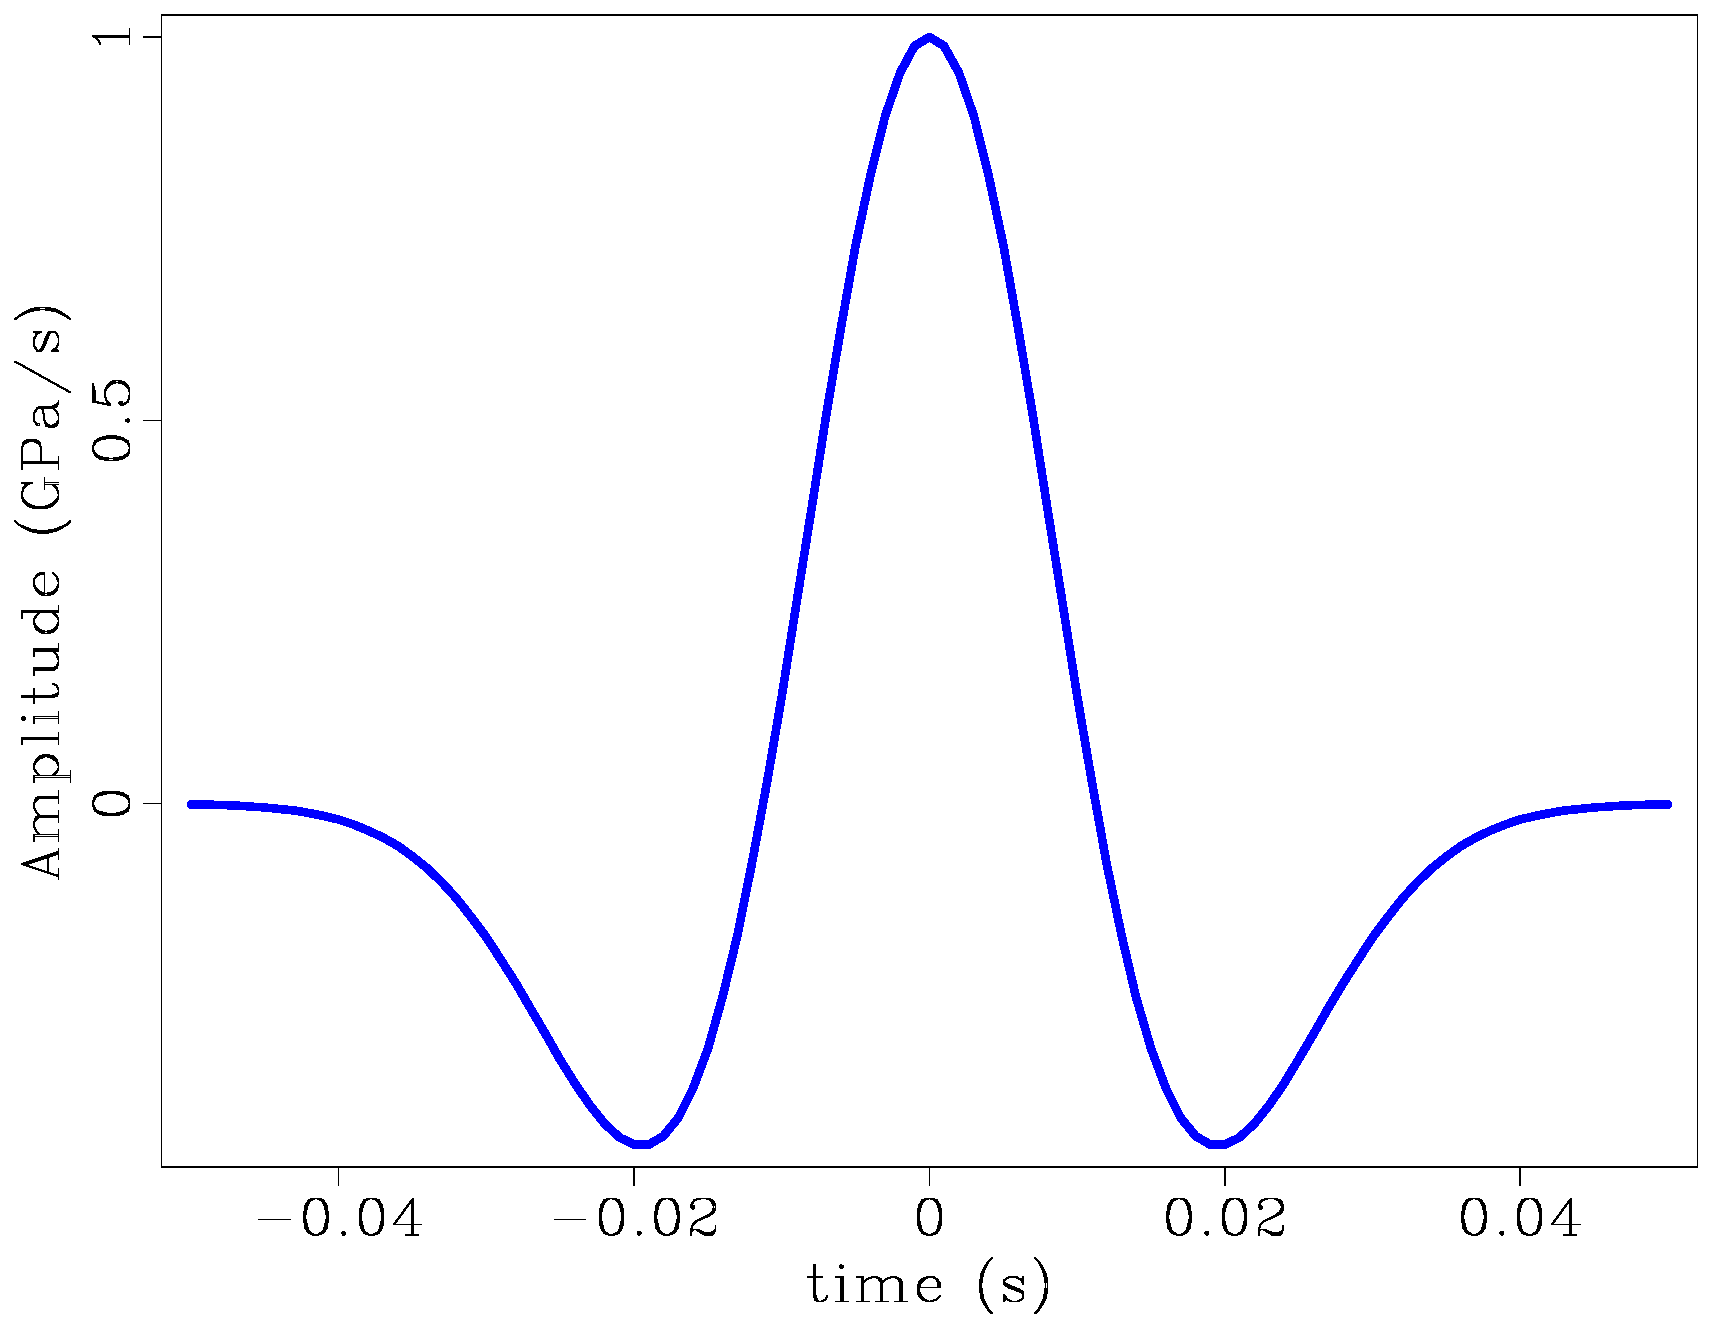
\includegraphics[width=\textwidth]{wavelet.pdf}
\caption{Ricker Wavelet, zero phase, 20 Hz center frequency}
\label{fig:wavelet}
\end{center}
\end{figure}

\begin{figure}[ht]   
\begin{center}
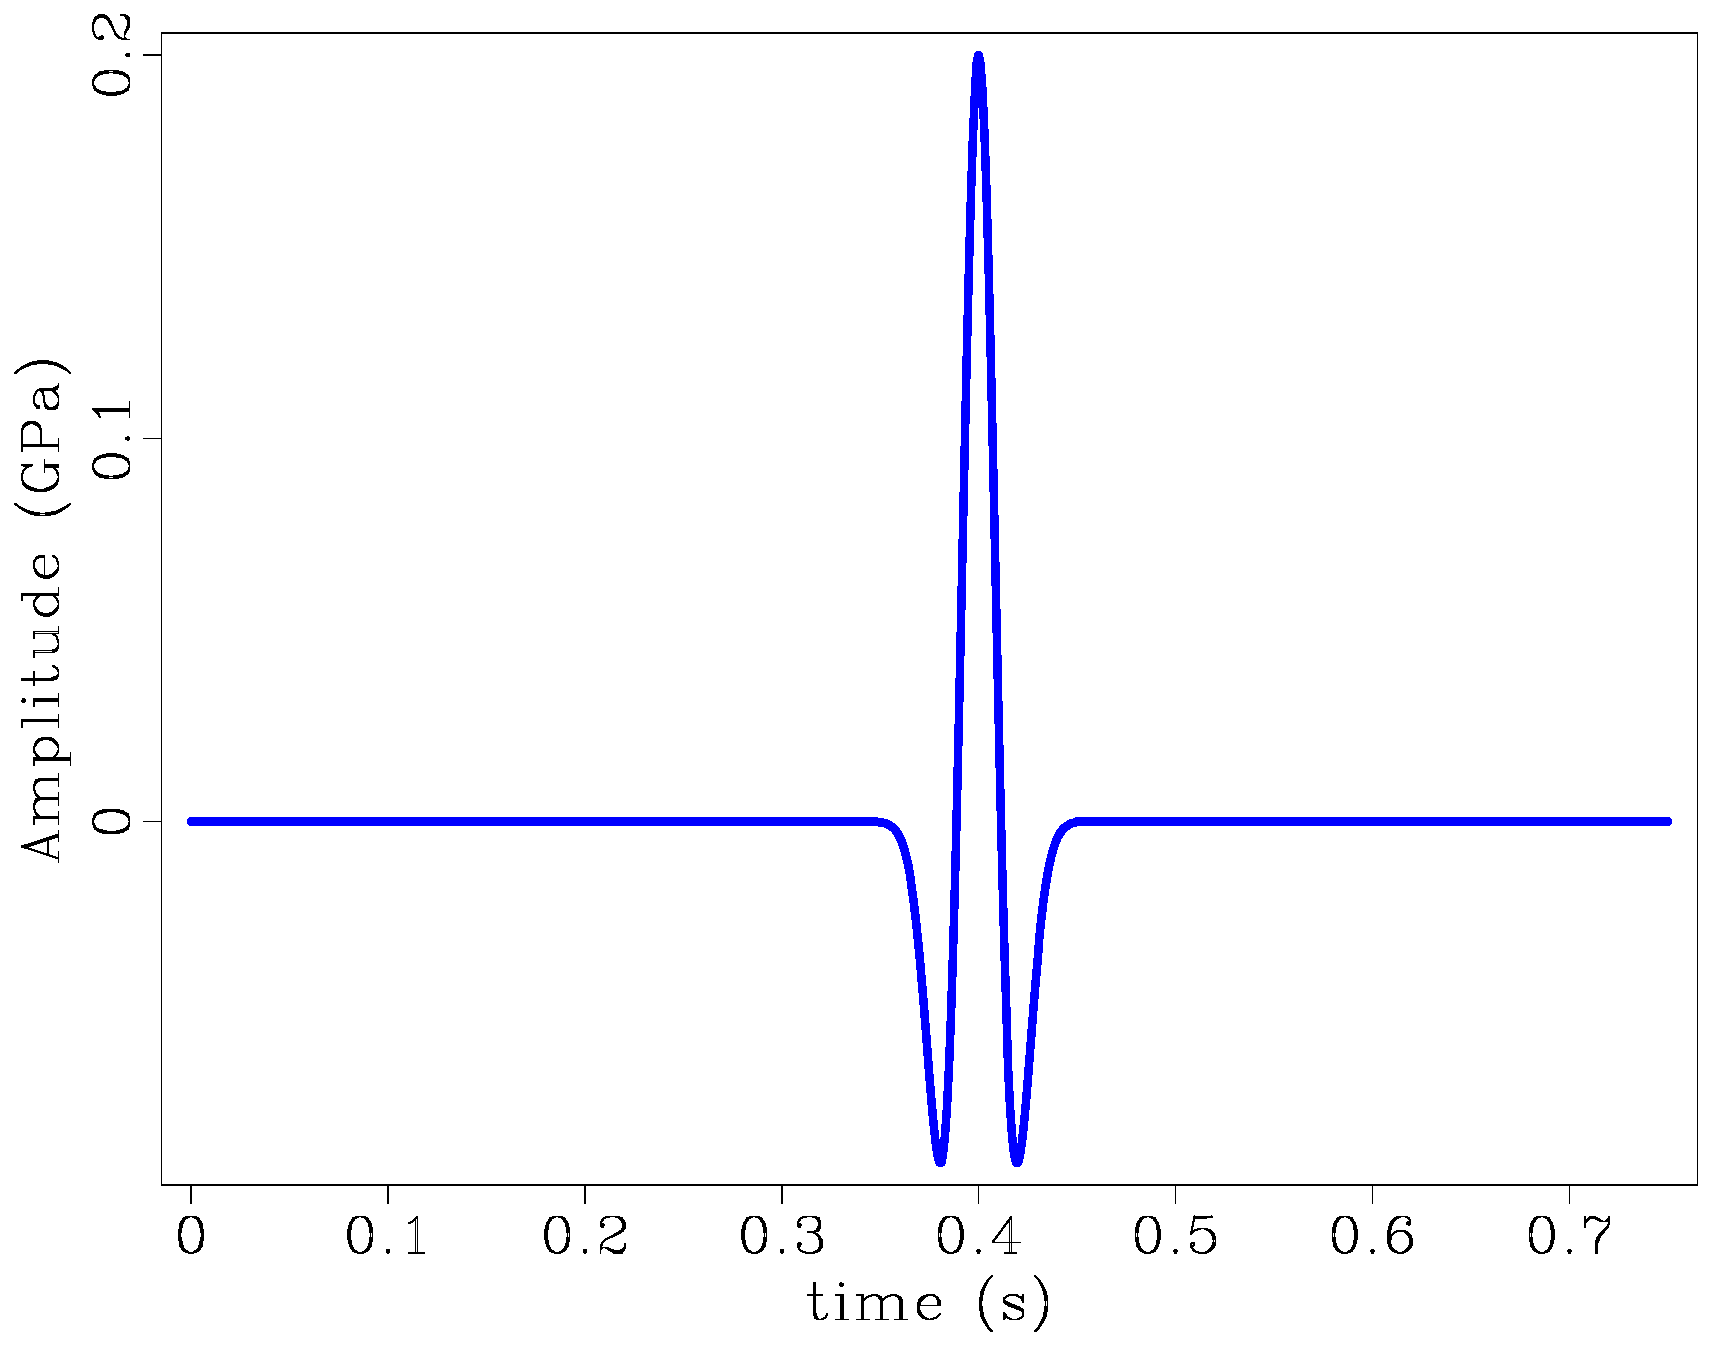
\includegraphics[width=\textwidth]{data.pdf}
\caption{Predicted data for 1D transmission 
  problem, source wavelet = 20 Hz Ricker wavelet of Figure 
  \ref{fig:wavelet}, source-receiver offset = 1 km, velocity = 2.5 
  km/s.}
\label{fig:data}
\end{center}
\end{figure}

\begin{figure}[ht]   
\begin{center}
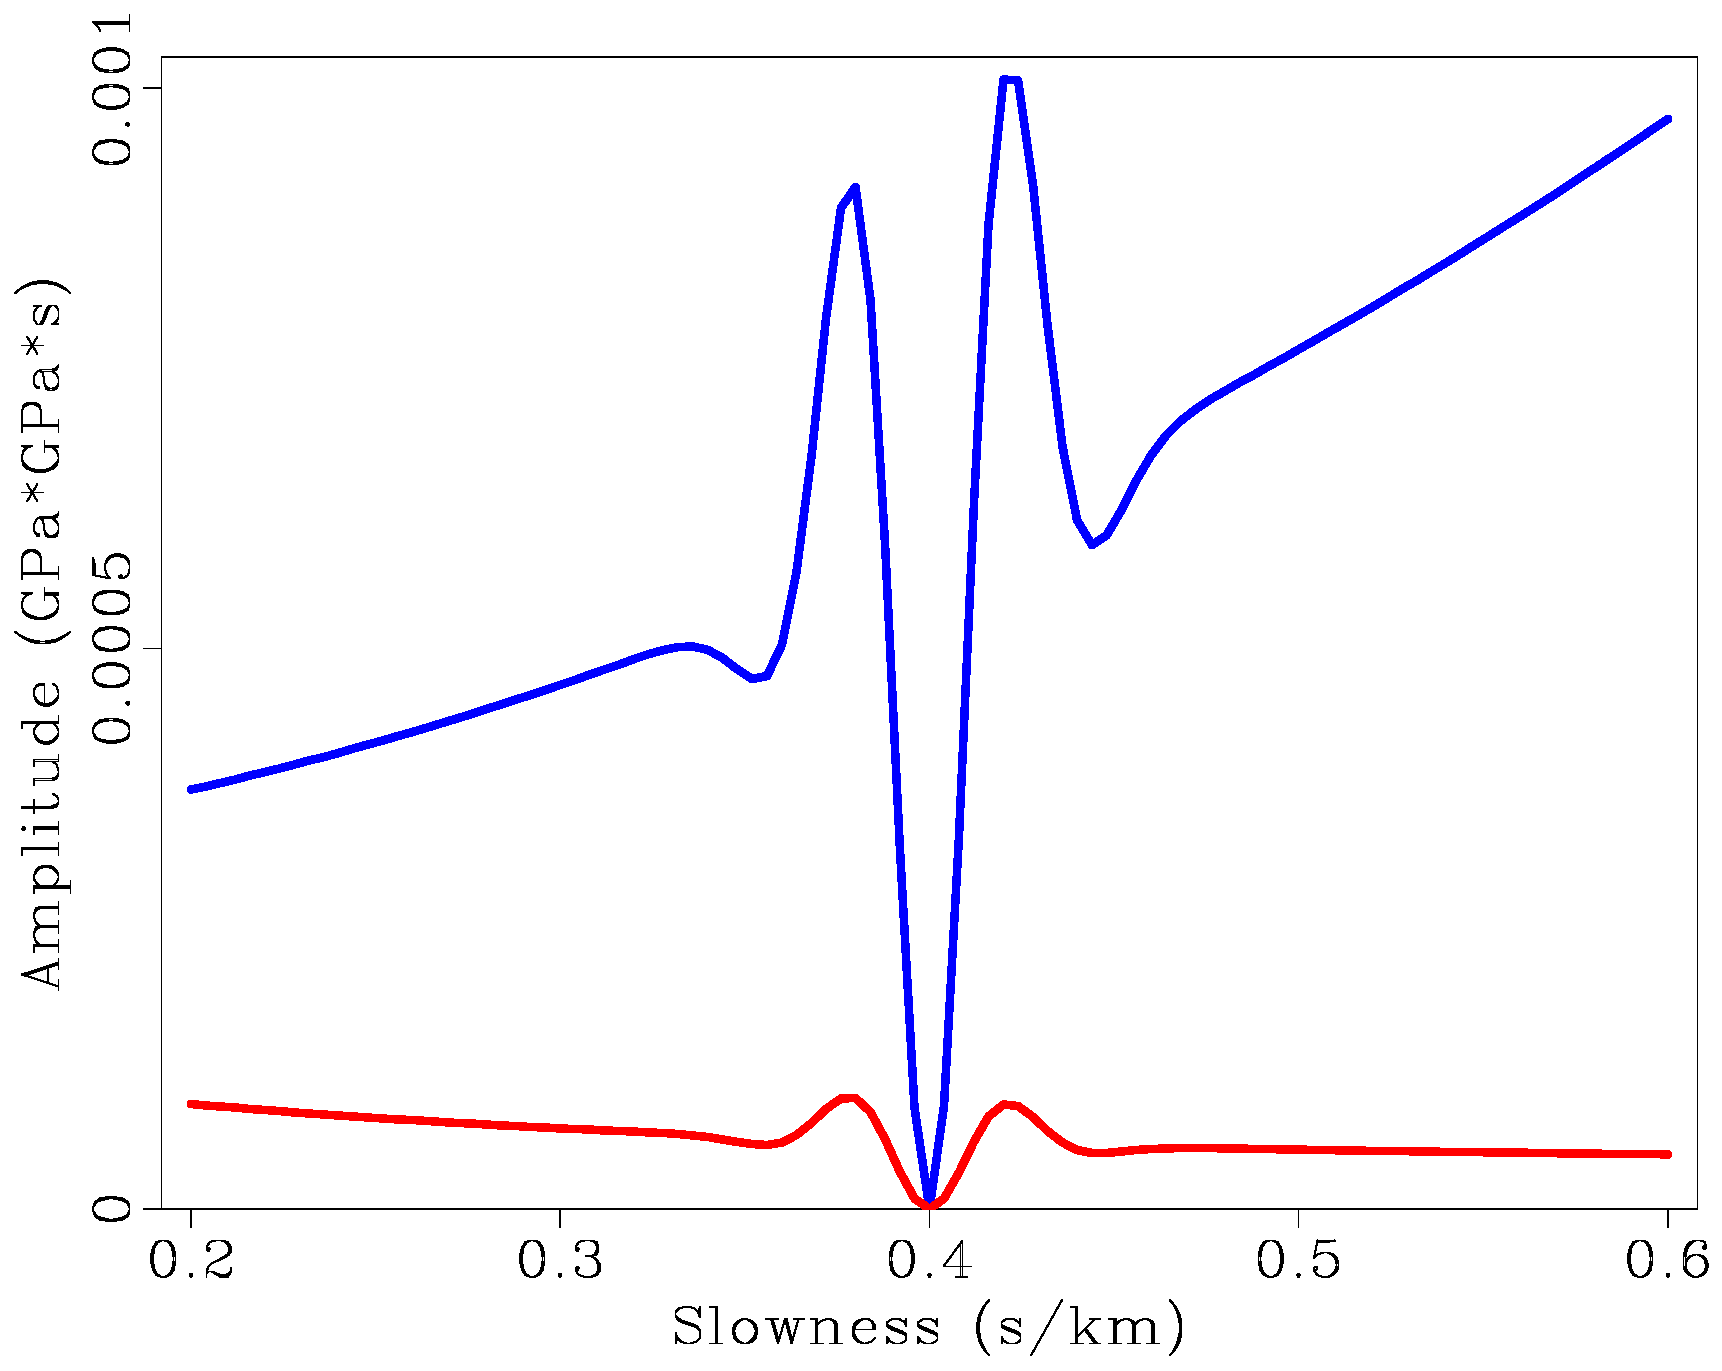
\includegraphics[width=\textwidth]{j0.pdf}
\caption{Blue curve = FWI objective, red curve =
  VPM-WRI objective, plotted as functions of slowness, $\alpha$= 0.1
  s/$\sqrt{\rm km}$.}
\label{fig:j0}
\end{center}
\end{figure}

\begin{figure}[ht]   
\begin{center}
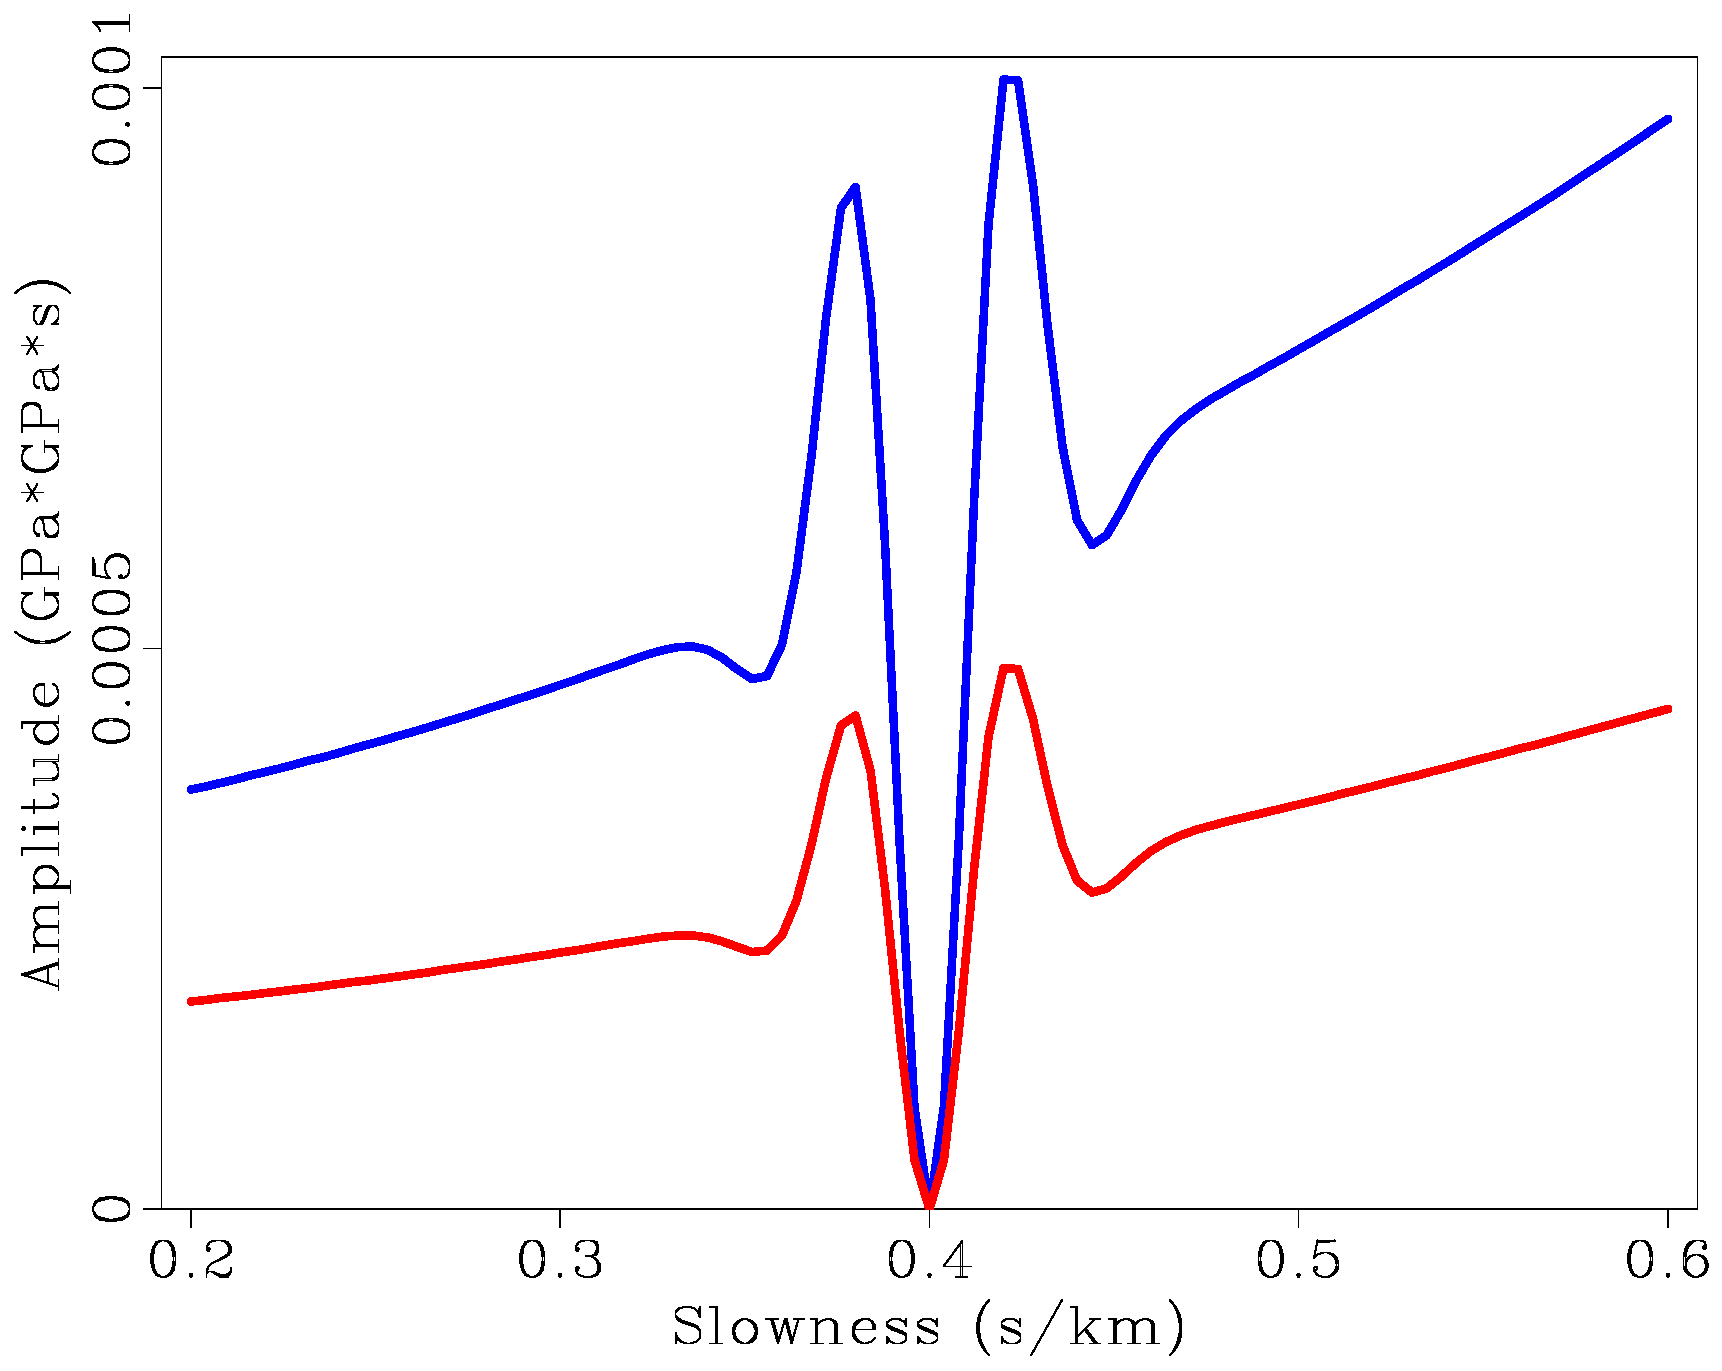
\includegraphics[width=\textwidth]{j3.pdf}
\caption{Blue curve = FWI objective, red curve =
  VPM-WRI objective, plotted as functions of slowness, $\alpha$= 1.0
  s/$\sqrt{\rm km}$.}
\label{fig:j3}
\end{center}
\end{figure}